% !TEX program = xelatex
% ============================================================================
% L_RAG Ablation Study -- ACL-style report entry point
%
% This file follows the official *ACL manuscript layout. Keep acl.sty and
% acl_natbib.bst from acl-org/acl-style-files available on the TeX path.
% Change [final] to [review] for an anonymized, line-numbered submission.
% ============================================================================
\documentclass[11pt]{article}
\usepackage[final]{acl}

% Standard ACL Unicode-capable template packages.
\usepackage{latexsym}
\usepackage{microtype}
\usepackage[english,bidi=default]{babel}
\babelfont{rm}{Times New Roman}
\usepackage{graphicx}

% Project-specific packages used by the section files.
\usepackage{amsmath,amssymb}
\usepackage{booktabs}
\usepackage{multirow}
\usepackage{tikz}
\usetikzlibrary{shapes.geometric, arrows, positioning}

\title{L\_RAG: A Controlled Ablation Study of Vietnamese Legal
Retrieval-Augmented Generation}

\author{
  Vu Khac Binh (23127029) \quad Van Thi Diem My (23127091) \\
  Tran Tuan Kiet (23127215) \quad Nguyen Le Thien Ly (23127223) \\
  Nguyen Phuong Thao (23127306) \\
  Faculty of Information Technology\\
  VNUHCM--University of Science
}

% The author block contains five student names, identifiers, and affiliation.
\setlength\titlebox{5cm}

\begin{document}
\maketitle

\begin{abstract}
This report evaluates design choices in L\_RAG, a Vietnamese legal
retrieval-augmented generation system, on a fixed 500-question benchmark
(400 answerable and 100 unanswerable questions). We report four controlled
ablation families rather than a pooled comparison: embedded chunk text,
dense versus hybrid retrieval with graph expansion, reranking within a shared
candidate pool, and Base versus chain-of-thought (CoT) prompting. Retrieval
is scored against gold chunk identifiers; lexical answer overlap,
template-based answerability behavior, structural citation fields, and
recorded latency are separate diagnostics. Metadata improves document success
at depth 10 by 4.5 percentage points but reduces MRR. The tested BM25+RRF
hybrid loses 5.98 Recall@10 points to dense retrieval and increases median
total latency from 5.483 to 31.538 seconds. One-hop graph expansion loses
11.81--12.40 Recall@10 points, chiefly by replacing seed evidence. In a
common 30-candidate pool, Jina reranking improves Recall@10 by 9.23 points
and nDCG@10 by 11.85 points over RRF-only. Under fixed context, CoT decreases
GPT-4o-mini Token F1 by 1.57 points. These are benchmark-bounded engineering
findings: lexical and structural diagnostics do not establish legal
correctness, citation entailment, or faithfulness.
\end{abstract}

% The report body is modular so each experiment can be updated without
% editing the ACL preamble or changing the paper's section order.
% ============================================================================
% Section 1: Introduction scaffold
% ============================================================================
\section{Introduction}
\label{sec:introduction}

\textit{Guidance: Introduce the Vietnamese legal QA problem, motivate
traceable evidence, and preview the report contributions. Keep this chapter
focused on why the problem matters; reserve implementation details for
Sections~\ref{sec:system-design} and~\ref{sec:implementation-setup}.}

\subsection{Background and Motivation}
\label{sec:intro-motivation}

\textit{Guidance: Add a motivating Vietnamese legal question, the governing
provision, and an explanation of why a cited answer is required. Include the
planned motivation figure and the keyword-search versus vector-RAG versus
L\_RAG contrast.}

\subsection{Problem Statement}
\label{sec:problem-statement}

\textit{Guidance: State the failure modes to be addressed: long documents,
hierarchy blindness, cross-document references, outdated provisions, missing
text, and unsupported answers. Add the problem-to-consequence table.}

\subsection{Project Objectives}
\label{sec:objectives}

\textit{Guidance: List measurable objectives and map each objective to an
implemented module, source file or script, and validation evidence. Add the
contribution map.}

\subsection{Scope of the System}
\label{sec:scope}

\textit{Guidance: Define the included corpus, preprocessing, graph, retrieval,
generation, and evaluation stages. Explicitly list excluded capabilities and
the assumptions that limit deployment.}

\subsection{Main Contributions}
\label{sec:contributions}

\textit{Guidance: Summarize the structured legal corpus, G-LRAG graph,
hybrid retrieval pipeline, citation-grounded generation, and controlled
ablation study. Use one contribution overview figure.}

\subsection{Report Organization}
\label{sec:report-organization}

\textit{Guidance: Explain the Problem $\rightarrow$ Data $\rightarrow$
Methodology $\rightarrow$ Implementation $\rightarrow$ Evaluation
$\rightarrow$ Ablations $\rightarrow$ Discussion $\rightarrow$ Conclusion
flow and add the report-roadmap figure.}

% ============================================================================
% Section 2: Background and Related Work scaffold
% ============================================================================
\section{Background and Related Work}
\label{sec:related-work}

\textit{Guidance: Replace these prompts with a focused literature review.
Explain which prior ideas motivate each L\_RAG design choice and identify the
gap addressed by the controlled ablations.}

\subsection{Retrieval-Augmented Generation}
\label{sec:related-rag}

\textit{Guidance: Define the standard query, retriever, context, prompt, LLM,
and answer pipeline. Add a standard RAG diagram and a grounding illustration.}

\subsection{Legal Information Retrieval}
\label{sec:related-legal-ir}

\textit{Guidance: Discuss authority, hierarchy, temporal validity, citation
dependencies, and the cost of retrieval errors in legal settings. Add the
legal-document hierarchy and a legal retrieval example.}

\subsection{Dense, Sparse, and Hybrid Retrieval}
\label{sec:related-hybrid}

\textit{Guidance: Compare dense retrieval, BM25, and rank fusion. Add the
retrieval comparison table and a vocabulary-mismatch example.}

\subsection{Knowledge-Graph-Augmented Retrieval}
\label{sec:related-graph}

\textit{Guidance: Explain how graph structure supplies containment,
neighboring, citation, amendment, and validity context. Add a graph-retrieval
illustration and a vector-versus-graph comparison table.}

\subsection{Reranking and Citation-Grounded Generation}
\label{sec:related-reranking}

\textit{Guidance: Introduce candidate reranking, cross-encoders, citation
grounding, and abstention. Add the two-stage ranking and citation-grounding
illustrations.}

\subsection{Design Requirements for Legal RAG}
\label{sec:related-requirements}

\textit{Guidance: Convert legal reliability requirements into design choices
and evaluation checks. Add a requirement traceability matrix and design
rationale diagram.}

% ============================================================================
% Section 3: Legal Dataset and Benchmark Construction scaffold
% ============================================================================
\section{Legal Dataset and Benchmark Construction}
\label{sec:dataset-construction}

\textit{Guidance: Describe the corpus and benchmark as reproducible data
products. Keep the running Vietnamese legal question consistent across the
dataset, graph, retrieval, and generation examples.}

\subsection{Legal Corpus and Raw Data Sources}
\label{sec:raw-corpus}

\textit{Guidance: Inventory raw files, record types, identifiers,
relationships, and text fields. Reuse the document-type distribution and add
a sanitized metadata and relationship example.}

\subsection{Dataset Normalization and Cleaning}
\label{sec:dataset-normalization}

\textit{Guidance: Document identifier, date, document-type, status, and
relationship transformations. Reuse the data-pipeline figure and add a
before-and-after record plus a normalization-rules table.}

\subsection{Relationship Processing and External References}
\label{sec:relationship-processing}

\textit{Guidance: Explain resolved in-corpus targets, unresolved external
targets, external stubs, relationship vocabulary, and direction verification.
Add the relationship-resolution diagram, vocabulary table, and stub example.}

\subsection{Quarantine and Data-Quality Verification}
\label{sec:quarantine}

\textit{Guidance: Show accepted records, quarantined records, verification
gates, final inclusion, audit counts, and reconciliation identities. Reuse the
edge-quarantine asset.}

\subsection{Legal Text Structuring}
\label{sec:text-structuring}

\textit{Guidance: Describe the Document $\rightarrow$ Provision $\rightarrow$
Chunk hierarchy and provenance pointers. Reuse the provision and chunk assets
and add the structured-artifact inventory.}

\subsection{QA Benchmark Construction}
\label{sec:benchmark-construction}

\textit{Guidance: Show context sampling, question generation, verification,
diversity filtering, deduplication, and final export. Add the benchmark-flow
figure, a record example, and stage-count table.}

\subsection{Question Categories and Answer Types}
\label{sec:question-taxonomy}

\textit{Guidance: Define single-hop, citation, legal-validity, multi-hop, and
cross-document categories, and relate them to abstractive, boolean,
extractive, and unanswerable answer types. Add the category-answer-type
matrix.}

\subsection{Ground-Truth Evidence}
\label{sec:ground-truth}

\textit{Guidance: Explain reference answers and document, provision, and chunk
identifiers. Add the evidence-link diagram, annotated JSONL record, and
ground-truth coverage table.}

\subsection{Dataset Statistics and Validation}
\label{sec:dataset-validation}

\textit{Guidance: Report corpus size, missing-text counts, orphan counts,
quarantine counts, external stubs, and reconciliation checks. Reuse the
length, node-type, and document-type assets and add a validation dashboard.}

% ============================================================================
% Section 4: L_RAG System Design and Methodology
% ============================================================================
\section{L\_RAG System Design and Methodology}
\label{sec:system-design}

L\_RAG turns the structured corpus and benchmark into an evidence-oriented
retrieval and generation pipeline. Offline processing creates normalized
records, graph artifacts, and vector or sparse indexes. Online processing
resolves query scope, retrieves candidate chunks, optionally expands or
filters them with the graph, reranks a bounded pool, and serializes the final
context for a citation-grounded generator. The same document, provision, and
chunk identifiers introduced in Section~\ref{sec:dataset-construction} are
carried through every stage.

\subsection{End-to-End System Architecture}
\label{sec:architecture}

The architecture has five operational phases: (1) query and temporal-scope
resolution, (2) dense and optional sparse retrieval, (3) graph filtering or
context expansion, (4) rank fusion and candidate reranking, and (5) prompt
construction, generation, and cited output. \hyperref[fig:architecture]{Figure~\ref*{fig:architecture}}
shows the data flow and the point at which each family of ablations changes a
component.

\begin{figure*}[t]
\centering
\resizebox{\textwidth}{!}{%
\begin{tikzpicture}[node distance=1.45cm, auto,
    block/.style={rectangle, draw=blue!80, fill=blue!5, thick, minimum width=3cm, minimum height=1cm, align=center, rounded corners},
    kgblock/.style={rectangle, draw=green!60!black, fill=green!5, thick, minimum width=3cm, minimum height=1cm, align=center, rounded corners},
    llmblock/.style={rectangle, draw=red!70, fill=red!5, thick, minimum width=3cm, minimum height=1cm, align=center, rounded corners},
    line/.style={draw, -latex', thick}]
    \node [block] (query) {User query $q$\\+(date/scope)};
    \node [block, right=1.3cm of query] (retrieve) {Dense E5\\+ optional BM25};
    \node [kgblock, below=1.15cm of retrieve] (graph) {G-LRAG overlay\\filter/expand};
    \node [block, right=1.3cm of retrieve] (fuse) {RRF and\\candidate mask};
    \node [block, right=1.3cm of fuse] (rank) {Cross-encoder\\reranking};
    \node [llmblock, below=1.15cm of rank] (generate) {Grounded prompt\\gpt-4o-mini};
    \node [block, left=1.3cm of generate] (output) {Answer +\\source citations};
    \path [line] (query) -- (retrieve);
    \path [line] (query) |- (graph);
    \path [line] (retrieve) -- (fuse);
    \path [line] (graph) -- (fuse);
    \path [line] (fuse) -- (rank);
    \path [line] (rank) -- (generate);
    \path [line] (generate) -- (output);
\end{tikzpicture}%
}%
\caption{End-to-end operational workflow of L\_RAG. The graph and reranker
stages are optional branches whose effects are tested under separate frozen
ablation controls.}
\label{fig:architecture}
\end{figure*}

The component boundaries are deliberate. The retriever decides which chunks
are available, the graph can alter that set under a fixed context budget, the
reranker only reorders a candidate pool, and the generator sees a serialized
top-10 context. This separation prevents a generation metric from being
mistaken for evidence-retrieval quality.

\subsection{Offline Data and Index Construction}
\label{sec:offline-construction}

Offline construction branches from the normalized records into three linked
artifacts. The structured-text branch emits provisions and chunks with stable
parent pointers. The graph branch emits document, provision, chunk, and
relationship nodes plus validity and authority metadata. The retrieval branch
embeds either chunk-only or header-plus-chunk text into a FAISS index and
builds tokenized BM25 shards for configurations that enable sparse retrieval.

The dense index uses L2-normalized vectors and inner-product search, which is
equivalent to cosine ranking for normalized embeddings. For the completed
hybrid runs, BM25 is built as 10 independent shards with shard-local IDF and
average-document-length statistics; shard candidates are merged by BM25 score
before RRF. The graph and index artifacts keep the same chunk IDs, so a
retrieved vector row can be joined back to its document and provision without
fuzzy matching. Frozen manifests record the corpus snapshot, model
checkpoint, index path, configuration name, and benchmark version used to
create each evaluation run.

\subsection{Online Query-Processing Workflow}
\label{sec:online-query}

At query time, the system first preserves the raw Vietnamese question and any
explicit date or scope constraint. The query encoder produces an E5 vector;
the dense branch retrieves a broad seed set, while the optional BM25 branch
searches tokenized shards. The branches are merged with RRF when hybrid mode
is enabled. In the completed retrieval/graph family, a graph variant keeps
the top five seeds, expands them within their parent provisions with
\texttt{max\_hop=1}, and replaces the baseline top-10 context with at most
ten expanded chunks. This is a complete context-selection policy: it uses
broad validity filtering and does not apply a query-time validity overlay or
reranking. The resulting candidates are trimmed to the family-specific
budget, reranked only in the reranker family, and serialized as the final
context.

Insufficient evidence follows an observable fallback path. If no candidate
survives a valid scope filter, if the context contains no usable text, or if
the prompt's evidence threshold is not met, the retrieval/graph prompt asks
the model to emit the Vietnamese fallback phrase
\textit{``Không có đủ thông tin trong ngữ cảnh được cung cấp.''}; the
fixed-context reasoning runs use the visible marker
\texttt{INSUFFICIENT\_CONTEXT}. These strings are saved for evaluation and
are not treated as proof that a question was legally unanswerable. Invalid
filters and unresolved external references remain visible in the run record
instead of being silently repaired.

\subsection{Knowledge Graph Construction}
\label{sec:graph-construction}

The G-LRAG graph uses Document ($D$), Provision ($P$), Chunk ($C$), and
ExternalStub nodes. Structural edges encode
\texttt{DOCUMENT\_HAS\_PROVISION}, \texttt{PROVISION\_HAS\_CHUNK},
\texttt{CHUNK\_NEXT}, and \texttt{PROVISION\_NEXT}. Legal-relation edges encode
citations, amendments, replacements, and repeals. Each edge retains source
provenance and is available to query-time traversal only after direction and
endpoint checks.

The overlay can fold validity fields relative to an \texttt{as\_of\_date}
parameter and can sort candidates by authority rank. A simplified precedence
ordering available to the system is
\begin{equation}
\text{Constitution} \succ \text{Law/Code} \succ
\text{Decree} \succ \text{Circular}.
\end{equation}
Reading-order traversal follows adjacent chunks or provisions to recover
nearby context; hop 1 covers the seed provision and additional hops reach
subsequent provisions. In the completed graph ablation, traversal is limited
to five seeds and at most ten retained chunks, with no query-time validity
overlay or reranking. This policy can replace strong seed evidence and is
therefore evaluated as a change to the candidate set, not as a free context
addition.

\subsection{Retrieval and Ranking}
\label{sec:retrieval-ranking}

The dense encoder is \texttt{intfloat/multilingual-e5-large}. For the
metadata condition, the indexed string is
\begin{equation}
\begin{aligned}
\text{Text}_{\mathrm{embed}}={}&\text{DocumentTitle}
\;\parallel\;\text{ProvisionHeader}\\
&\;\parallel\;\text{ChunkContent}.
\end{aligned}
\end{equation}
the chunk-only condition removes the first two fields. The FAISS index uses
\texttt{IndexFlatIP}. Sparse retrieval uses \texttt{rank\_bm25} with
\texttt{underthesea} tokenization and $k_1=1.5$, $b=0.75$. Dense and sparse
lists are fused by
\begin{equation}
\mathrm{RRF}(d)=\sum_{m\in\{\mathrm{dense},\mathrm{BM25}\}}
\frac{1}{60+r_m(d)}.
\end{equation}

The dense/hybrid/graph family retrieves 50 seeds and retains at most ten final
chunks. The reranker family reconstructs a common RRF pool of 30 candidates
($C_{30}$), then retains ten ($T_{10}$). mMiniLM, Qwen3, BGE, and Jina score
the full query--candidate pair with a cross-encoder. Models are loaded,
executed, and unloaded sequentially to avoid GPU memory interference. The
reranker can improve ordering inside $C_{30}$, but it cannot recover evidence
that never entered the pool.

\subsection{Answer Generation}
\label{sec:answer-generation}

The context serializer writes each retained chunk with its chunk ID, document
title, provision header, and passage text. All generators use temperature
$0.0$, but output limits are family-specific: the retrieval/graph runs set no
explicit client-side token cap, while the fixed-context reasoning comparison
uses a 1,024-token limit. The retrieval/graph prompt asks for Vietnamese
answers and uses the fallback phrase
\textit{``Không có đủ thông tin trong ngữ cảnh được cung cấp.''} when the
evidence is insufficient; the reasoning runs use the visible marker
\texttt{INSUFFICIENT\_CONTEXT}. A citation should identify the governing
article or instrument.

The observable output record contains the final answer, citation markers,
parser fields, refusal marker, latency, and the ordered context IDs. It does
not contain hidden chain-of-thought, reasoning-token accounting, or a human
claim-entailment annotation. Consequently, the evaluation can report output
format and lexical overlap but cannot infer legal correctness from a fluent
answer or a well-formed citation.

\subsection{End-to-End Worked Example}
\label{sec:worked-example}

Consider a benchmark question asking whether a specified land-use action is
permitted under a named Vietnamese instrument. The source record is first
joined to its document ID and effective date. Its controlling article is
represented as a provision, and the provision is split into ordered chunks
whose IDs remain linked to the parent. The query encoder retrieves candidate
chunks; the graph can add the adjacent clause or a cited instrument; RRF and
the reranker order the retained candidates; and the serializer presents the
top ten with their provenance.

The generator then produces an answer in the requested format and attaches
the document and provision identifiers used as citations. If the retrieved
context contains only a related definition but not the operative condition,
the intended output is \texttt{INSUFFICIENT\_CONTEXT}. The example illustrates
why the report distinguishes document success from exact chunk recall and
citation presence from citation entailment: each is a different observable
stage in the same traceable workflow.

% ==========================================================================
% Section 5: Implementation and Experimental Setup
% ==========================================================================
\section{Implementation and Experimental Setup}
\label{sec:implementation-setup}

This section states the controls and scoring rules needed to interpret the
ablations in Section~\ref{sec:ablation-study}. The experiment families share
a benchmark but are not a single factorial experiment: candidate pools,
context construction, and latency accounting differ. Variants are therefore
compared only within their own controlled family.

\subsection{Pipeline and Frozen Artifacts}
\label{sec:software-architecture}

The evaluated pipeline has five stages: query embedding with
\texttt{intfloat/multilingual-e5-large}; dense FAISS retrieval and, where
enabled, tokenized BM25 retrieval; RRF fusion, graph expansion, or
cross-encoder reranking; serialization of retained chunks into a grounded
prompt; and answer generation and evaluation. The analysis reads frozen
manifests, predictions, aggregate metrics, latency records, and error logs;
it does not rerun models. Every primary comparison is joined by
\texttt{qa\_id}, so an aggregate difference is traceable to paired cases.

\subsection{Indexes, Graph, and Runtime Settings}
\label{sec:build-process}

The dense/hybrid/graph experiment uses a FAISS index with 1,513,376 chunk
vectors and a graph over the same number of chunks. The hybrid branch searches
ten BM25 shards. Dense/hybrid retrieval uses a 50-result search budget, broad
filtering, a final context of 10 chunks, and RRF parameter $k=60$ where BM25
is enabled. Graph variants take five seeds, traverse one hop, and retain at
most 10 graph-context chunks. The dense/hybrid and reranker generation
artifacts use GPT-4o-mini.

The reranker family fixes a 30-chunk RRF candidate pool (C30) and a 10-chunk
final context (T10), comparing no reranking, RRF-only, mMiniLM, Qwen3, BGE,
and Jina. The primary generator study compares GPT-4o-mini Base and CoT with
the saved top-10 context fixed by question. The metadata study changes only
the indexed string from chunk body to header-plus-chunk text; encoder, FAISS,
top-$k=10$, generator, prompt, seed, corpus, and benchmark stay fixed.

\subsection{Benchmark and Metrics}
\label{sec:evaluation-metrics}

The benchmark contains 500 questions: 400 answerable questions with gold
chunk identifiers and 100 unanswerable questions. Retrieval scores use only
the 400 answerable records. Given gold chunks $G$ and retrieved top-$k$ chunks
$R_k$, context recall is $|G \cap R_k|/|G|$; Hit@k indicates that at least one
gold chunk occurs. MRR and nDCG reward early gold rank. Candidate Recall@30 is
the evidence ceiling for the reranker study and is intentionally identical
for every reranker.

Exact Match, Token F1, and ROUGE-L are lexical overlap with reference answers.
The saved unanswerable score is a refusal-marker diagnostic, not a semantic
assessment of legal appropriateness. Citation presence and structural coverage
measure saved marker/parser fields, not claim-to-source entailment. Latency is
reported as saved p50/p95 timing; cached-BM25 reranker timing is not full
online sparse-retrieval timing.

\subsection{Pairing, Uncertainty, and Claim Boundaries}
\label{sec:experimental-protocol}

Headline effects are paired by \texttt{qa\_id}. Retrieval uses the shared
answerable intersection; scheduled-denominator answerability diagnostics keep
all 500 cases. Percentile paired-bootstrap confidence intervals use 10,000
resamples for headline metadata, dense/hybrid, reranker, and GPT comparisons;
reranker slices use 2,000. Intervals crossing zero are reported as
inconclusive. The non-GPT prompt pairs are descriptive when code provenance,
timeouts, retries, or retrieved context differ.

No blinded legal-correctness labels, claim-level faithfulness labels, or
validated semantic judge are available. Thus, no result is interpreted as
proof of legal correctness, legal safety, citation entailment, or faithful
reasoning merely because it improves a lexical, rank, citation-format, or
refusal-format metric.

% ============================================================================
% Section 6: Ablation Studies
% ============================================================================
\section{Ablation Studies}
\label{sec:ablation-study}

We report five completed ablation analyses
grouped into four run families: embedding text; dense, hybrid, and graph
retrieval as one joint retrieval/graph family; reranking; and generator
prompting. Comparisons are made within a family because candidate
construction, context budgets, output limits, and latency accounting differ;
the results are not treated as one pooled factorial experiment.

\subsection{Embedding Text Ablation: Chunk-Only versus Chunk+Metadata}
\label{sec:ablation-chunk-meta}

This comparison holds the dense encoder, generator, benchmark, seed, and raw
FAISS evaluation path fixed. Only the indexed text changes from the chunk body
to a header-plus-chunk representation. On 400 paired answerable questions,
exact chunk Recall@10 is effectively unchanged: both variants round to
48.5\%, with an unrounded metadata-minus-chunk-only difference of only
+0.08 percentage points (reported as +0.1 pp in
\hyperref[tab:embedding-results]{Table~\ref*{tab:embedding-results}}).
Metadata nevertheless increases document-level success at rank 10 from
65.8\% to 70.2\%, a paired gain of +4.5 pp (95\% CI [+0.5,+8.8]), while
MRR@10 decreases by 5.9 pp (95\% CI [$-9.1,-2.7$]).

Because the metadata representation includes both document titles and
provision headers, we additionally report provision-level success. At rank
10, provision success is 53.8\% for chunk-only retrieval and 53.5\% for
chunk+metadata, a negligible $-0.25$ pp difference (95\% CI
[$-5.0,+4.5$]). At rank 5, provision success decreases from 44.3\% to
40.3\%. Thus, the observed metadata gain is concentrated at document
discovery rather than provision identification or exact chunk ranking. The
retrieval curves and paired outcomes are shown in
\hyperref[fig:embedding-ablation]{Figure~\ref*{fig:embedding-ablation}}.

\begin{figure*}[t]
\centering
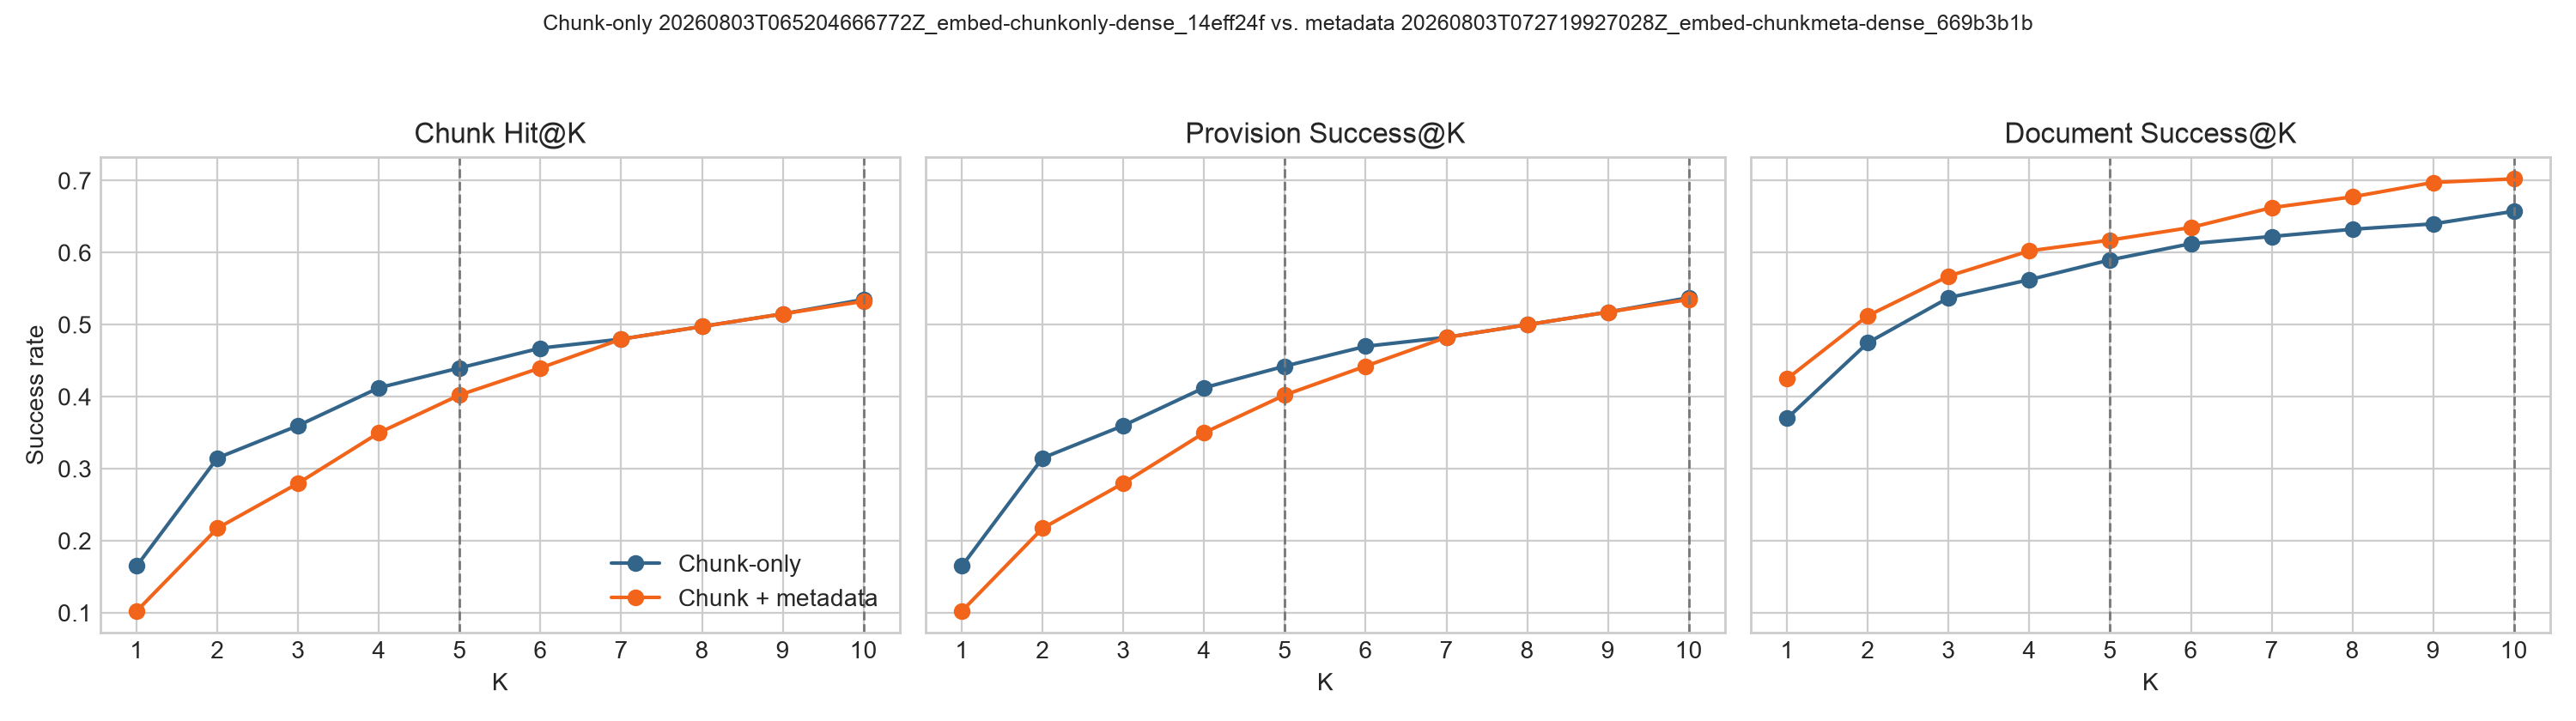
\includegraphics[width=0.48\textwidth]{../../ablation_study/chunkOnly_vs_chunkMetadata/results/success_at_k_curve.png}
\hfill
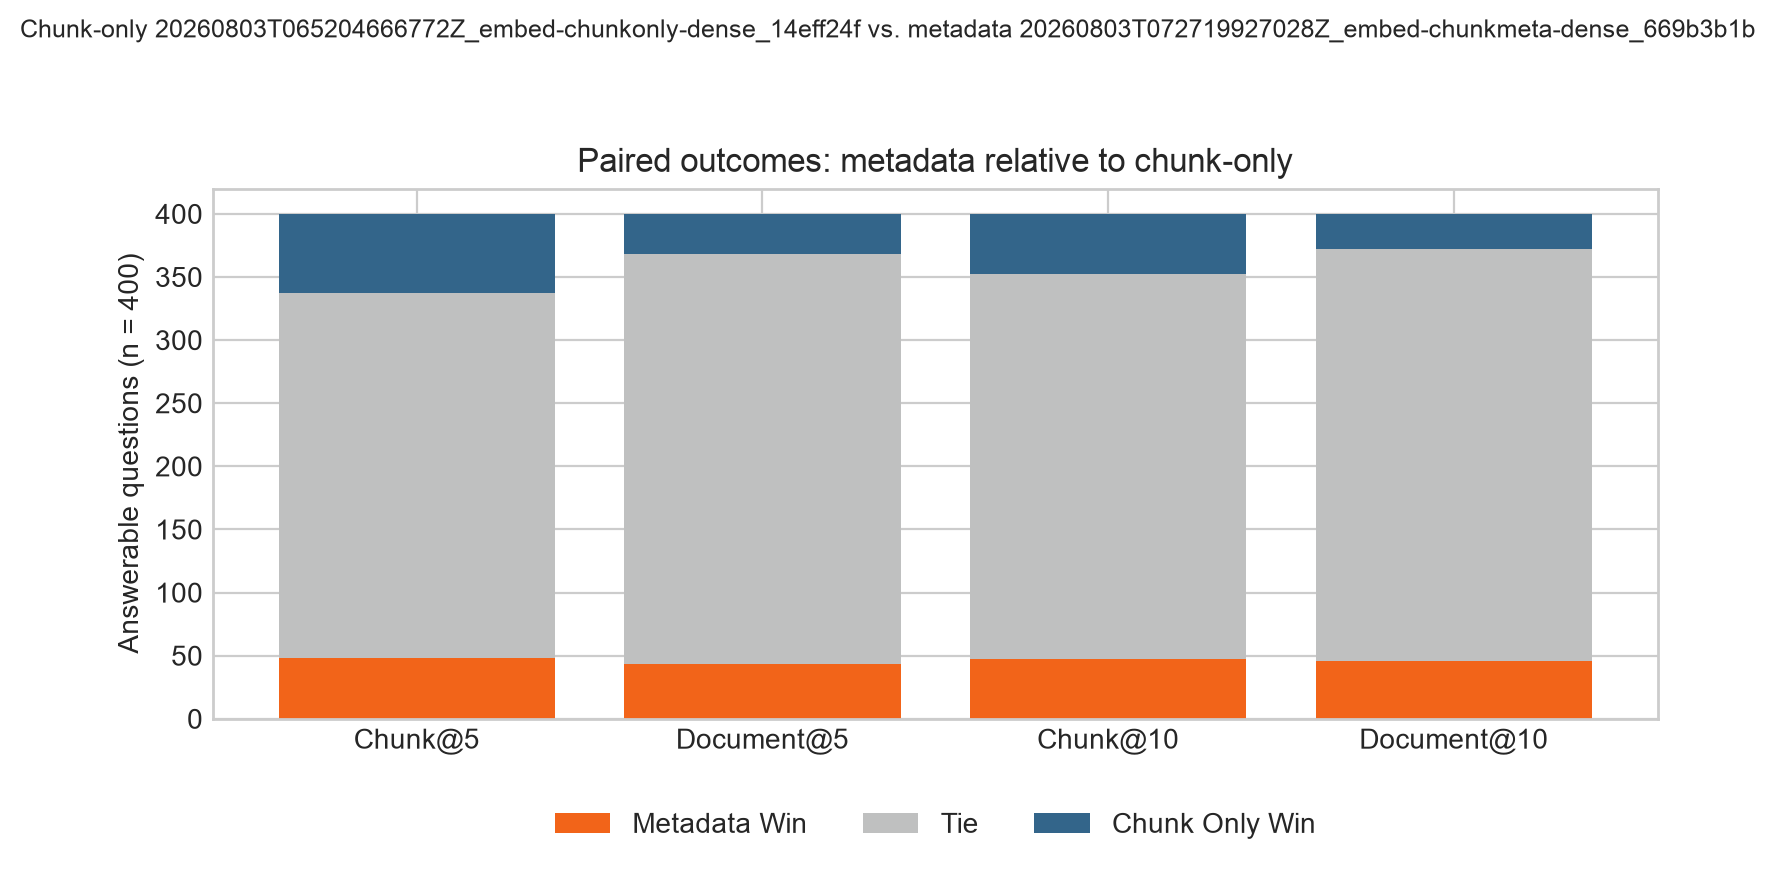
\includegraphics[width=0.48\textwidth]{../../ablation_study/chunkOnly_vs_chunkMetadata/results/paired_win_tie_loss.png}
\caption{Embedding-text ablation diagnostics. The left panel shows success
curves by retrieval depth; the right panel shows paired win, tie, and loss
counts. Both plots use the shared answerable-question comparison.}
\label{fig:embedding-ablation}
\end{figure*}

\begin{table*}[t]
\centering
\scriptsize
\caption{Embedding-text ablation on 400 paired answerable questions. Values
are percentages. Document and provision success denote retrieval of at least one
chunk from a gold document or gold provision, respectively. Deltas are
chunk+metadata minus chunk-only. Recall@10 values in the two rows both round
to 48.5\%; the unrounded difference is +0.08 pp.}
\label{tab:embedding-results}
\resizebox{\textwidth}{!}{%
\begin{tabular}{lrrrrrrrrrr}
\toprule
\textbf{Variant} & \textbf{Hit@5} & \textbf{Recall@5} & \textbf{MRR@5} &
\textbf{Doc@5} & \textbf{Prov@5} & \textbf{Hit@10} &
\textbf{Recall@10} & \textbf{MRR@10} & \textbf{Doc@10} &
\textbf{Prov@10} \\
\midrule
Chunk-only & 44.0 & 39.0 & 27.4 & 59.0 & 44.3 & 53.5 & 48.5 & 28.6 & 65.8 & 53.8 \\
Chunk+metadata & 40.2 & 36.8 & 20.9 & 61.8 & 40.3 & 53.2 & 48.5 & 22.7 & 70.2 & 53.5 \\
Delta & $-3.8$ & $-2.2$ & $-6.5$ & $+2.8$ & $-4.0$ & $-0.2$ &
$+0.1$ & $-5.9$ & $+4.5$ & $-0.3$ \\
\bottomrule
\end{tabular}%
}
\end{table*}
\subsection{Retrieval Ablation: Dense versus Hybrid Retrieval}
\label{sec:ablation-retrieval}

The dense/hybrid comparison uses the same header-plus-chunk dense index,
50-seed retrieval budget, 10-chunk final context, benchmark, and generator.
Hybrid retrieval adds ten sharded BM25 indexes and reciprocal rank fusion.
DenseOnly outperforms
HybridOnly on Recall@10 (48.55\% versus 42.57\%) and nDCG@10 (0.2813 versus
0.2638); the full comparison is in
\hyperref[tab:dense-hybrid-results]{Table~\ref*{tab:dense-hybrid-results}}.
The paired Recall@10 difference is $-5.98$ points with a 95\% CI of
[$-9.71,-2.21$]. Hybrid retrieval also raises recorded total median latency
from 5.483 seconds to 31.538 seconds. The hybrid total includes 26.990 seconds
per query amortized from 13,495 seconds of BM25 batch precomputation over the
500-question batch; this accounting is distinct from online request latency.
Paired uncertainty is reported in
\hyperref[tab:dense-hybrid-paired]{Table~\ref*{tab:dense-hybrid-paired}}.

\begin{table*}[t]
\centering
\scriptsize
\caption{Dense versus hybrid retrieval. Retrieval values use 400 answerable
questions; latency percentiles use all 500 cases. The fallback column is the
fraction of 100 unanswerable outputs containing the family-specific Vietnamese
fallback phrase.}
\label{tab:dense-hybrid-results}
\resizebox{\textwidth}{!}{%
\begin{tabular}{lrrrrrrr}
\toprule
\textbf{Method} & \textbf{Recall@5} & \textbf{Recall@10} &
\textbf{MRR@10} & \textbf{nDCG@10} & \textbf{Retrieval p50/p95} &
\textbf{Total p50/p95} & \textbf{Fallback} \\
\midrule
DenseOnly & 0.3678 & 0.4855 & 0.2267 & 0.2813 & 0.797/0.856 & 5.483/9.946 & 0.38 \\
HybridOnly & 0.3140 & 0.4257 & 0.2252 & 0.2638 & 27.855/27.924 & 31.538/33.623 & 0.38 \\
\bottomrule
\end{tabular}%
}
\end{table*}

\begin{table}[t]
\centering
\scriptsize
\caption{Paired hybrid-minus-dense differences.}
\label{tab:dense-hybrid-paired}
\begin{tabular}{lrr}
\toprule
\textbf{Metric} & \textbf{Mean delta} & \textbf{95\% CI} \\
\midrule
Recall@10 & $-0.0598$ & $[-0.0971,-0.0221]$ \\
MRR@10 & $-0.0015$ & $[-0.0299,+0.0271]$ \\
nDCG@10 & $-0.0175$ & $[-0.0437,+0.0085]$ \\
\bottomrule
\end{tabular}
\end{table}

\subsection{Graph Ablation: With versus Without Graph Expansion}
\label{sec:ablation-graph}

Graph variants expand the top five seed chunks within their parent provisions
with \texttt{max\_hop=1}, replace the baseline top-10 context, and retain at
most 10 chunks. They use broad validity filtering without a query-time
validity overlay or reranking, so this comparison evaluates the complete
context-selection policy rather than graph traversal in isolation. Graph
expansion currently displaces more evidence than it adds.
Relative to DenseOnly, DenseGraph changes Recall@10 by $-12.40$ points and
loses at least one previously retrieved gold chunk for 61 questions while
adding a graph-only gold chunk for only one question. The HybridOnly to
HybridGraph change is $-11.81$ points, with 59 questions losing a gold chunk
and six gaining one; the displacement counts and rank deltas are summarized in
\hyperref[tab:graph-effect]{Table~\ref*{tab:graph-effect}}.

Graph contexts are denser because they contain fewer chunks on average (5.605
for DenseGraph and 6.305 for HybridGraph), and their identity precision is
higher. This is a precision--coverage trade-off, not evidence of an overall
retrieval-quality improvement. Of the 65 gold-chunk occurrences lost by
DenseGraph, 60 were outside the original top-five seeds; for HybridGraph, 52
of 60 were outside the original top five. The counts support seed-preserving
expansion as the next controlled graph test.

\begin{table*}[t]
\centering
\scriptsize
\caption{Effect of graph expansion on top-10 gold evidence. Counts are over
400 answerable questions; graph-only gold is introduced by expansion and
graph-missed gold was present before expansion but absent afterward. The
fallback column is the fraction of 100 unanswerable outputs containing the
family-specific Vietnamese fallback phrase.}
\label{tab:graph-effect}
\resizebox{\textwidth}{!}{%
\begin{tabular}{lrrrrrrrr}
\toprule
\textbf{Base} & \textbf{$\Delta$ Recall@10} & \textbf{$\Delta$ MRR@10} &
\textbf{$\Delta$ nDCG@10} & \textbf{Graph-only gold} &
\textbf{Graph-missed gold} & \textbf{Avg. chunks} & \textbf{ID precision} &
\textbf{Fallback} \\
\midrule
DenseOnly $\rightarrow$ DenseGraph & $-0.1240$ & $-0.0222$ & $-0.0439$ &
1 query (0.25\%) & 61 queries (15.25\%) & 5.605 & 0.0800 & 0.41 \\
HybridOnly $\rightarrow$ HybridGraph & $-0.1181$ & $-0.0240$ & $-0.0411$ &
6 queries (1.50\%) & 59 queries (14.75\%) & 6.305 & 0.0641 & 0.47 \\
\bottomrule
\end{tabular}%
}
\end{table*}

\subsection{Reranker Ablation}
\label{sec:ablation-reranking}

The reranker family compares no reranking, RRF-only, mMiniLM, Qwen3, BGE,
and Jina over a reconstructed shared RRF pool of 30 candidates and a final
top 10. All six runs cover the same 500 questions without retrieval or
generation errors, and the reconstruction matches the recorded RRF-only
top-10 prefix for 500/500 questions. Candidate Recall@30 is 0.5995 and
Candidate Hit@30 is 0.6450 for every configuration, so the comparison measures
ranking and retention within a fixed evidence ceiling.

Jina is the strongest retrieval configuration: relative to RRF-only, it
improves Recall@10 by +9.23 points, MRR@10 by +13.35 points, and nDCG@10 by
+11.85 points; all three 95\% paired-bootstrap intervals exclude zero. Qwen3
and BGE also have positive intervals, while mMiniLM supplies a smaller
positive gain at the lowest reranker cost. BGE has the highest token F1 and
ROUGE-L, whereas Jina has the highest observed unanswerable accuracy. These
answer metrics are lexical and abstention diagnostics, not legal correctness
judgments. Aggregate scores and latency are linked in
\hyperref[tab:reranker-results]{Table~\ref*{tab:reranker-results}}, with
paired effects in \hyperref[tab:reranker-paired]{Table~\ref*{tab:reranker-paired}}
and diagnostic curves in \hyperref[fig:reranker-curves]{Figure~\ref*{fig:reranker-curves}}.

\begin{table*}[t]
\centering
\scriptsize
\caption{Multi-reranker ablation over a shared 30-candidate pool and final
top-10 context. Retrieval and overlap values are means over 400 answerable
questions; recorded unanswerable accuracy and p50 latency use the complete
500-case runs.}
\label{tab:reranker-results}
\resizebox{\textwidth}{!}{%
\begin{tabular}{lrrrrrrrrr}
\toprule
\textbf{Model} & \textbf{Recall@10} & \textbf{Hit@10} & \textbf{MRR@10} &
\textbf{nDCG@10} & \textbf{Token F1} & \textbf{ROUGE-L} &
\textbf{Unans. acc.} & \textbf{Rerank p50} & \textbf{Total p50} \\
\midrule
None & 0.4842 & 0.5375 & 0.2167 & 0.2714 & 0.2801 & 0.2453 & 0.856 & 0.000 & 2.925 \\
RRF-only & 0.4382 & 0.4800 & 0.2335 & 0.2728 & 0.2750 & 0.2416 & 0.874 & 0.000 & 2.972 \\
mMiniLM & 0.4973 & 0.5425 & 0.3047 & 0.3425 & 0.2901 & 0.2568 & 0.872 & 0.385 & 3.343 \\
Qwen3 & 0.5218 & 0.5725 & 0.3418 & 0.3688 & 0.2912 & 0.2583 & 0.876 & 9.695 & 13.007 \\
BGE & 0.5188 & 0.5675 & 0.3247 & 0.3593 & \textbf{0.2955} & \textbf{0.2603} & 0.868 & 2.872 & 5.848 \\
Jina & \textbf{0.5305} & \textbf{0.5850} & \textbf{0.3670} &
\textbf{0.3914} & 0.2913 & 0.2558 & \textbf{0.884} & 1.278 & \textbf{4.158} \\
\bottomrule
\end{tabular}%
}
\end{table*}

\begin{table*}[t]
\centering
\scriptsize
\caption{Paired effects of each reranker relative to RRF-only. Deltas are in
percentage points; intervals are 95\% percentile bootstrap CIs from 10,000
question-level resamples over the 400 answerable cases. A negative false
refusal delta indicates fewer refusals on answerable questions.}
\label{tab:reranker-paired}
\resizebox{\textwidth}{!}{%
\begin{tabular}{lrrrr}
\toprule
\textbf{Reranker} & \textbf{$\Delta$ Recall@10} & \textbf{$\Delta$ MRR@10} &
\textbf{$\Delta$ nDCG@10} & \textbf{$\Delta$ false refusal} \\
\midrule
mMiniLM & $+5.91$ [$+1.85,+9.96$] & $+7.12$ [$+3.55,+10.68$] &
$+6.96$ [$+3.77,+10.26$] & $+0.25$ [$-3.00,+3.50$] \\
Qwen3 & $+8.37$ [$+4.57,+12.25$] & $+10.84$ [$+7.24,+14.36$] &
$+9.60$ [$+6.52,+12.73$] & $-0.25$ [$-3.25,+2.75$] \\
BGE & $+8.07$ [$+4.29,+11.80$] & $+9.12$ [$+5.50,+12.70$] &
$+8.65$ [$+5.47,+11.84$] & $+0.75$ [$-2.25,+3.75$] \\
Jina & $+9.23$ [$+5.51,+12.98$] & $+13.35$ [$+9.51,+17.24$] &
$+11.85$ [$+8.46,+15.27$] & $-1.25$ [$-4.00,+1.25$] \\
\bottomrule
\end{tabular}%
}
\end{table*}

\begin{figure*}[t]
\centering
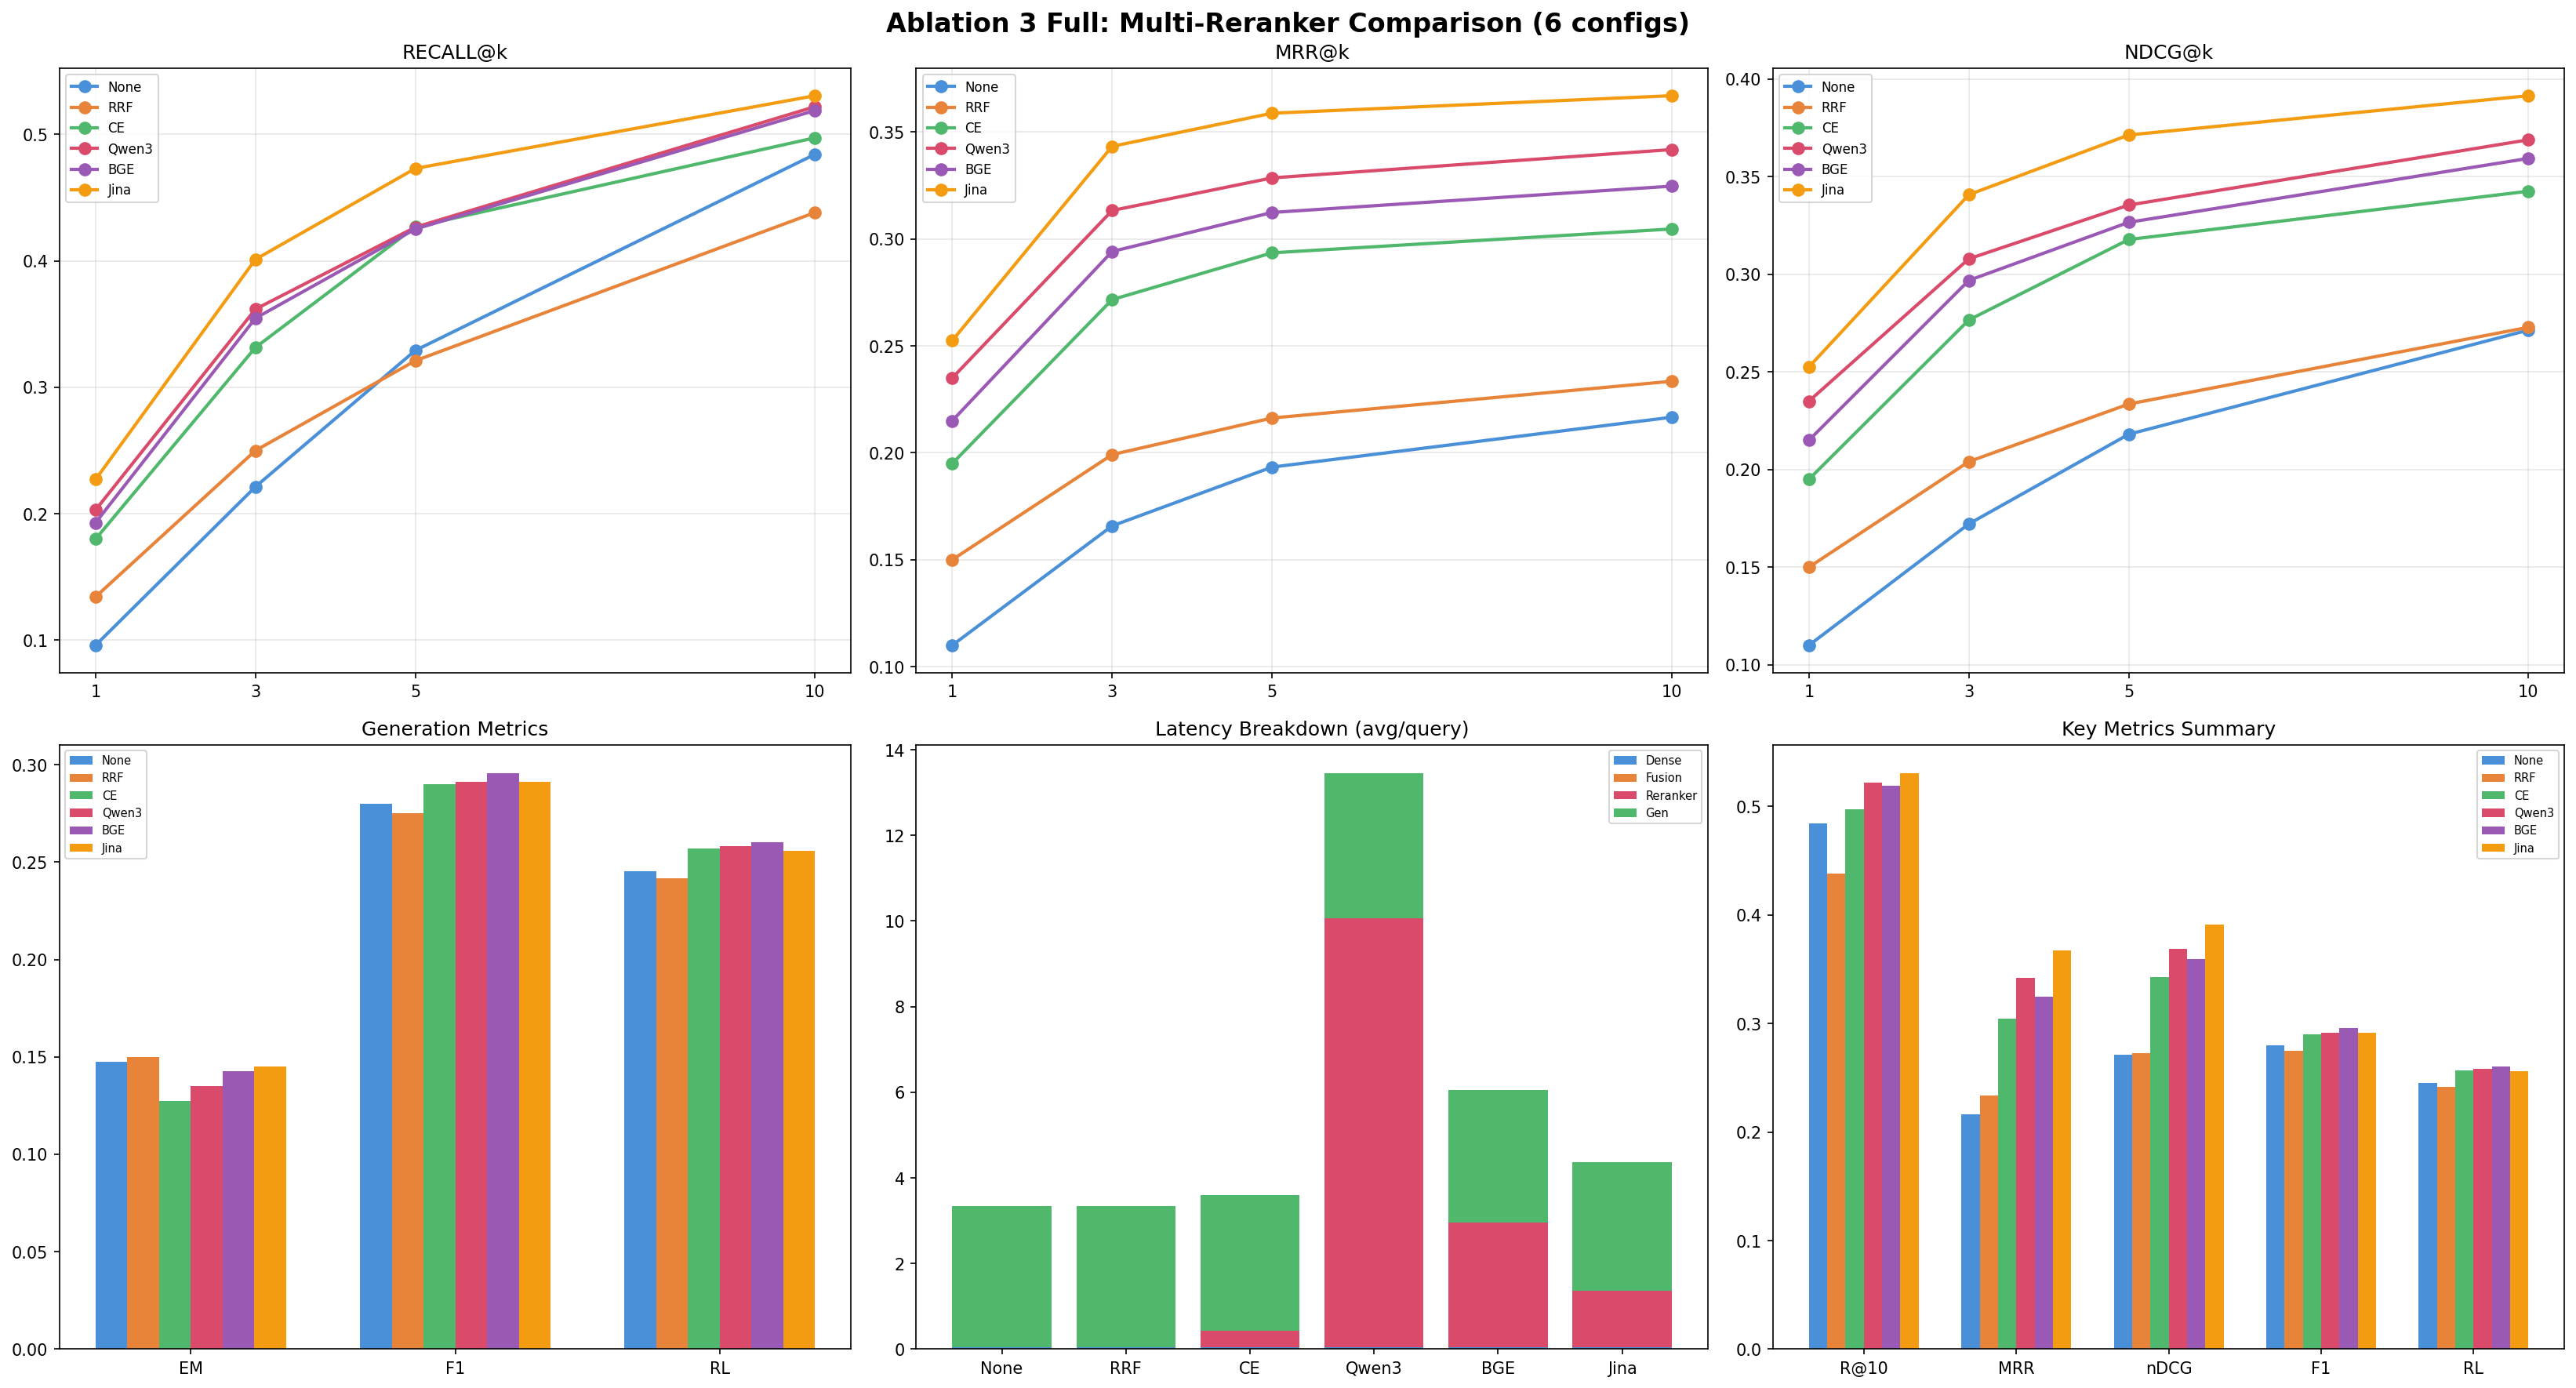
\includegraphics[width=\textwidth]{../../ablation_work/reranker_choices/evaluation_runs/ablation3_reranker_v2/charts.png}
\caption{Reranker curves, answer-overlap diagnostics, latency breakdown, and
headline metrics from the six-configuration run. The paired confidence
intervals in Table~\ref{tab:reranker-paired} are the primary uncertainty
analysis.}
\label{fig:reranker-curves}
\end{figure*}

\subsection{Generator Ablation: Base Prompt versus Chain-of-Thought Prompt}
\label{sec:ablation-reasoning}

The generator-reasoning family keeps the intended retrieved top-10 context
fixed for each question and changes the prompt mode. The primary comparison
uses complete GPT-4o-mini Base and CoT runs: both cover all 500 benchmark
questions and share 400 answerable question IDs. The frozen artifacts report
zero retrieval-context mismatches. The DeepSeek-V3.1-Thinking, GLM-5, and
Qwen3-8B pairs are complete but descriptive; four shared DeepSeek cases have
different exact top-10 chunk-ID sequences, and the Qwen pair uses different
code snapshots, timeout values, and retry limits.

On the 400 paired answerable questions, CoT decreases Token F1 from 24.72\% to
23.15\% ($-1.57$ points) and ROUGE-L from 21.60\% to 19.90\% ($-1.71$
points). Exact match is essentially unchanged (14.00\% to 13.75\%,
$-0.25$ points). The Token F1 win/tie/loss count is 79/164/157 in favor of
Base. The run inventory is in
\hyperref[tab:llm-reasoning-runs]{Table~\ref*{tab:llm-reasoning-runs}} and the
paired GPT-4o-mini result is linked in
\hyperref[tab:llm-reasoning-paired]{Table~\ref*{tab:llm-reasoning-paired}}.

\begin{table*}[t]
\centering
\scriptsize
\caption{End-to-end generator-reasoning run inventory. Lexical metrics are
means over successful answerable cases; decision accuracy is the saved
template-based answerability diagnostic.}
\label{tab:llm-reasoning-runs}
\resizebox{\textwidth}{!}{%
\begin{tabular}{lllrrrrr}
\toprule
\textbf{Model} & \textbf{Prompt} & \textbf{Run directory} & \textbf{Valid/500} &
\textbf{EM (\%)} & \textbf{Token F1 (\%)} & \textbf{ROUGE-L (\%)} &
\textbf{Decision acc. (\%)} \\
\midrule
GPT-4o-mini & Base & \texttt{4o-mini-base} & 500/500 & 14.00 & 24.72 & 21.60 & 82.60 \\
GPT-4o-mini & CoT & \texttt{4o-mini-CoT} & 500/500 & 13.75 & 23.15 & 19.90 & 84.00 \\
DeepSeek-V3.1-Thinking & Base & \texttt{deepseek-base} & 500/500 & 22.25 & 17.84 & 15.28 & 92.00 \\
DeepSeek-V3.1-Thinking & CoT & \texttt{deepseek-CoT} & 500/500 & 22.25 & 16.51 & 14.12 & 92.20 \\
GLM-5 & Base & \texttt{glm5-base} & 500/500 & 25.25 & 16.91 & 14.90 & 91.80 \\
GLM-5 & CoT & \texttt{glm5-CoT} & 500/500 & 25.00 & 16.23 & 14.27 & 93.40 \\
Qwen3-8B & Base & \texttt{qwen3-8b-base} & 500/500 & 19.25 & 21.98 & 18.92 & 95.80 \\
Qwen3-8B & CoT & \texttt{qwen3-8b-CoT} & 500/500 & 17.25 & 20.05 & 17.17 & 95.20 \\
\bottomrule
\end{tabular}%
}
\end{table*}

\begin{table*}[t]
\centering
\scriptsize
\caption{Primary paired GPT-4o-mini Base-versus-CoT comparison on 400
answerable questions. Deltas are CoT minus Base in percentage points; CIs
are percentile bootstrap intervals from 10,000 paired resamples.}
\label{tab:llm-reasoning-paired}
\resizebox{\textwidth}{!}{%
\begin{tabular}{lrrrr}
\toprule
\textbf{Metric} & \textbf{Base (\%)} & \textbf{CoT (\%)} &
\textbf{$\Delta$ (pp)} & \textbf{95\% paired CI (pp)} \\
\midrule
Exact Match & 14.00 & 13.75 & $-0.25$ & $[-1.50,+1.00]$ \\
Token F1 & 24.72 & 23.15 & $-1.57$ & $[-2.24,-0.92]$ \\
ROUGE-L & 21.60 & 19.90 & $-1.71$ & $[-2.34,-1.10]$ \\
\bottomrule
\end{tabular}%
}
\end{table*}

\subsection{Jina vs RRF-Only by Question Category and Answer Type}
\label{sec:breakdown-analysis}

This subgroup analysis is restricted to the 400 answerable questions and
compares Jina against RRF-only within the shared reranker candidate pool.
Consequently, the slice counts differ from the full benchmark inventory in
Section~\ref{sec:question-taxonomy}, which also includes 100 unanswerable
questions. The largest observed gains occur for legal-validity and citation
questions. The extractive and multi-hop slices have wider intervals, and the
cross-document and hard subsets are too small for stable subgroup estimates.
The reported intervals use 2,000 paired-bootstrap resamples; see
\hyperref[tab:jina-slices]{Table~\ref*{tab:jina-slices}}.

\begin{table*}[t]
\centering
\scriptsize
\caption{Jina versus RRF-only on selected answerable category and answer-type
slices. Counts differ from the full benchmark inventory because unanswerable
questions are excluded. Deltas are percentage points with 95\%
paired-bootstrap CIs.}
\label{tab:jina-slices}
\resizebox{\textwidth}{!}{%
\begin{tabular}{llrlll}
\toprule
\textbf{Dimension} & \textbf{Slice} & \textbf{$n$} &
\textbf{$\Delta$ Recall@10} & \textbf{$\Delta$ MRR@10} &
\textbf{$\Delta$ nDCG@10} \\
\midrule
Category & citation & 106 & $+11.89$ [$+2.82,+21.70$] &
$+16.22$ [$+7.86,+24.51$] & $+15.82$ [$+7.51,+23.82$] \\
Category & legal validity & 91 & $+14.47$ [$+6.96,+21.43$] &
$+18.90$ [$+10.28,+27.26$] & $+15.22$ [$+9.13,+21.50$] \\
Category & single hop & 172 & $+5.04$ [$-0.00,+10.37$] &
$+9.63$ [$+4.34,+14.69$] & $+8.41$ [$+3.81,+13.05$] \\
Category & multi hop & 20 & $+7.50$ [$-0.83,+17.50$] &
$+10.12$ [$-3.42,+24.33$] & $+7.95$ [$-0.77,+17.98$] \\
Answer type & extractive & 78 & $+0.13$ [$-8.85,+9.74$] &
$+8.53$ [$-0.90,+17.39$] & $+7.14$ [$-1.33,+16.23$] \\
Answer type & abstractive & 199 & $+13.65$ [$+8.50,+18.80$] &
$+14.74$ [$+9.61,+20.14$] & $+13.81$ [$+9.56,+18.71$] \\
Answer type & boolean & 123 & $+7.86$ [$+1.63,+14.50$] &
$+14.18$ [$+7.64,+21.13$] & $+11.68$ [$+6.27,+17.95$] \\
\bottomrule
\end{tabular}%
}
\end{table*}

The category pattern suggests that reranking is most useful when relevant
evidence must be distinguished among several semantically related legal
passages, as in citation and validity questions. However, these are subgroup
analyses rather than separate preregistered experiments, so differences
between slices are treated descriptively rather than as evidence of
between-category effects.

\subsection{Evidence Coverage, Abstention, and Citation Analysis}
\label{sec:evidence-analysis}

The GPT-4o-mini pair provides structural diagnostics for evidence availability,
answerability decisions, and citations. These fields describe observable
output format and saved parser coverage; they do not establish citation
entailment, semantic refusal quality, or legal correctness. CoT lowers the
false-refusal rate on answerable questions from 21.25\% to 19.50\%, while
unanswerable recognition remains 98.00\% for both prompts. Citation presence
rises from 78.25\% to 81.00\% and mean unique sources from 1.46 to 1.68, but
structural citation coverage falls from 89.42\% to 87.91\%; the detailed
diagnostics are in \hyperref[tab:evidence-diagnostics]{Table~\ref*{tab:evidence-diagnostics}}.

\begin{table*}[t]
\centering
\scriptsize
\caption{Structural evidence, abstention, and citation diagnostics for the
paired GPT-4o-mini runs.}
\label{tab:evidence-diagnostics}
\resizebox{\textwidth}{!}{%
\begin{tabular}{lrrl}
\toprule
\textbf{Diagnostic} & \textbf{Base} & \textbf{CoT} & \textbf{Interpretation} \\
\midrule
Citation presence & 78.25\% & 81.00\% & at least one marker on answerable output \\
Structural coverage & 89.42\% & 87.91\% & saved factual-sentence marker share \\
Mean unique sources & 1.46 & 1.68 & structural source count \\
False refusal (answerable) & 21.25\% & 19.50\% & refusal-marker diagnostic \\
Unanswerable recognition & 98.00\% & 98.00\% & refusal-marker diagnostic \\
\bottomrule
\end{tabular}%
}
\end{table*}

Evidence-stratified deltas do not reverse the result: CoT Token F1 is lower
when all gold support is retrieved ($-1.98$ points, $n=138$), when support is
partial ($-1.86$ points, $n=29$), and when support is absent ($-1.30$ points,
$n=233$). The saved records cannot support claim-level faithfulness.

\begin{table*}[t]
\centering
\scriptsize
\caption{Evidence-availability strata for the paired GPT-4o-mini reasoning
comparison. Values are lexical means on the 400 paired answerable cases.}
\label{tab:llm-reasoning-evidence}
\resizebox{\textwidth}{!}{%
\begin{tabular}{lrrrrrrr}
\toprule
\textbf{Evidence stratum} & \textbf{$n$} & \textbf{Base F1} &
\textbf{CoT F1} & \textbf{$\Delta$ F1} & \textbf{Base ROUGE-L} &
\textbf{CoT ROUGE-L} & \textbf{$\Delta$ ROUGE-L} \\
\midrule
Support fully retrieved & 138 & 28.24 & 26.26 & $-1.98$ & 25.64 & 23.34 & $-2.30$ \\
Partial support retrieved & 29 & 25.62 & 23.76 & $-1.86$ & 21.04 & 19.45 & $-1.59$ \\
No support retrieved & 233 & 22.53 & 21.23 & $-1.30$ & 19.29 & 17.92 & $-1.37$ \\
\bottomrule
\end{tabular}%
}
\end{table*}

\subsection{Latency and Efficiency Comparison}
\label{sec:ablation-efficiency}

Latency values are interpreted only within their measurement scope. The
retrieval/graph family records retrieval-stage and total latency, but the
Hybrid rows include 26.990 seconds per query amortized from a 13,495-second
BM25 batch computation over 500 questions. They therefore combine an offline
batch cost with measured query-time work rather than representing direct
online request latency. Reranker timings are cached-stage measurements over a
preconstructed candidate pool and exclude full online sparse retrieval. The
generator rows measure generation under the fixed-context reasoning family.
Accordingly, the rows in
\hyperref[tab:latency-results]{Table~\ref*{tab:latency-results}} should not be
read as a single end-to-end latency leaderboard across families.

Within the reranker family, mMiniLM has the lowest recorded reranking p50,
followed by Jina, BGE, and Qwen3. Within the generator family, CoT raises
generation p50/p95 from 2.92/5.74 seconds to 3.68/6.17 seconds and total
p50/p95 from 13.99/17.21 to 14.74/18.42 seconds. Reranker p95, peak GPU
memory, and controlled full-online throughput are unavailable. Hardware,
batching, warm-up/cache policy, and model-load inclusion are not recorded
consistently across all run families, so the report makes no
hardware-normalized cross-family efficiency claim.

\begin{table*}[t]
\centering
\scriptsize
\caption{Recorded latency by measurement scope. Values are p50/p95 seconds
unless noted. Rows from different scopes are not directly comparable.
Reranker p95 was not recorded.}
\label{tab:latency-results}
\resizebox{\textwidth}{!}{%
\begin{tabular}{llll}
\toprule
\textbf{Configuration} & \textbf{Stage p50/p95} &
\textbf{Total p50/p95} & \textbf{Measurement scope} \\
\midrule
DenseOnly & 0.797/0.856 & 5.483/9.946 & measured retrieval + total \\
DenseGraph & 0.798/0.860 & 4.998/9.750 & measured retrieval/graph + total \\
HybridOnly & 27.855/27.924 & 31.538/33.623 & measured + amortized BM25 batch cost \\
HybridGraph & 27.858/27.929 & 31.180/33.312 & measured + amortized BM25 batch cost \\
\midrule
mMiniLM & 0.385/N/A & 3.343/N/A & cached candidate-pool reranking \\
Jina & 1.278/N/A & 4.158/N/A & cached candidate-pool reranking \\
BGE & 2.872/N/A & 5.848/N/A & cached candidate-pool reranking \\
Qwen3 & 9.695/N/A & 13.007/N/A & cached candidate-pool reranking \\
\midrule
GPT-4o-mini Base & 2.92/5.74 & 13.99/17.21 & fixed-context generation \\
GPT-4o-mini CoT & 3.68/6.17 & 14.74/18.42 & fixed-context generation \\
\bottomrule
\end{tabular}%
}
\end{table*}

\subsection{Aggregate Failure Modes and Representative Examples}
\label{sec:qualitative-ablation}
The aggregate results reveal several recurring failure modes. Metadata can improve document-level discovery while degrading exact evidence ranking, and graph-based context construction can displace already retrieved gold evidence under a fixed context budget. The following per-question traces illustrate how these retrieval changes propagate to generated answers.

\paragraph{Metadata can demote the governing evidence.}
\textbf{QA ID:} \texttt{vlrag-e6094add97}. \

\textbf{Question:} ``Có cần chuẩn bị giấy tờ gì đặc biệt không khi tôi là lãnh đạo một sở tại tỉnh Tiền Giang muốn đi nước ngoài?'' \

\textbf{Reference:} ``Khi đi nước ngoài, bạn phải có văn bản xin ý kiến Ủy ban nhân dân tỉnh trước khi tiến hành các thủ tục liên quan.'' \

\textbf{Chunk-only:} Gold chunk is ranked 1. \
\textbf{Generated answer:} ``Có. Là lãnh đạo sở, bạn cần có văn bản xin ý kiến Ủy ban nhân dân tỉnh trước khi tiến hành các thủ tục liên quan [1].'' \

\textbf{Chunk+metadata:} The same gold chunk falls to rank 9. \
\textbf{Generated answer:} ``Bạn cần chuẩn bị các giấy tờ sau khi đi nước ngoài về việc công: văn bản đề nghị của cơ quan, đơn vị; văn bản chấp thuận của tổ chức Đảng nếu là đảng viên; công văn, thư mời hoặc giấy triệu tập; và các thông tin về mục đích, thời gian, nước đến và nguồn kinh phí [1][2][4].'' \

\textbf{Effect:} MRR@10 decreases from $1.000$ to $0.111$, while Token F1 decreases from $0.750$ to $0.234$. The gold evidence remains in the top-10 context, but higher-ranked related provisions dominate the generated answer. This case shows that metadata can improve broader document matching without improving the rank of the exact governing provision.

\paragraph{Graph context can displace already retrieved evidence.}
\textbf{QA ID:} \texttt{vlrag-bbca4159cf}. \

\textbf{Question:} ``Gia đình tôi tham gia thực hiện đề tài khoa học xã hội cấp tỉnh, xin hỏi những ai có trách nhiệm phải thi hành quyết định về việc đánh giá, nghiệm thu đề tài này?'' \

\textbf{Reference:} ``Chánh Văn phòng Ủy ban nhân dân tỉnh; Giám đốc Sở Khoa học và Công nghệ; thủ trưởng các sở, ban, ngành; Chủ tịch Ủy ban nhân dân các huyện, thị xã; các đơn vị liên quan; và các tổ chức, cá nhân thực hiện đề tài.'' \

\textbf{HybridOnly:} Gold chunk is retrieved at rank 9. \
\textbf{Generated answer:} ``Những người có trách nhiệm thi hành quyết định về việc đánh giá, nghiệm thu đề tài khoa học xã hội cấp tỉnh bao gồm: Chánh Văn phòng Ủy ban nhân dân tỉnh, Giám đốc Sở Khoa học và Công nghệ, thủ trưởng các sở, ban, ngành cấp tỉnh, Chủ tịch Ủy ban nhân dân các huyện, thị, thành phố, cùng các tổ chức và cá nhân có liên quan. Căn cứ: Điều 3 của Quyết định 11/2009/QĐ-UBND.'' \

\textbf{HybridGraph:} The final context no longer contains the gold chunk, and no useful graph neighbor replaces it. \
\textbf{Generated answer:} ``Sở Khoa học và Công nghệ tỉnh có trách nhiệm tổ chức hướng dẫn, đôn đốc, kiểm tra các tổ chức, cá nhân tham gia thực hiện đề tài, dự án khoa học xã hội và nhân văn cấp tỉnh. Ngoài ra, Hội đồng đánh giá, nghiệm thu cấp tỉnh cũng có trách nhiệm trong việc đánh giá và nghiệm thu đề tài. Căn cứ: Quyết định 11/2009/QĐ-UBND và Quyết định 89/2005/QĐ-UB.'' \

\textbf{Effect:} Recall@10 decreases from $1.0$ to $0.0$, MRR@10 from $0.111$ to $0$, and Token F1 from $0.560$ to $0.286$. This is a direct seed-displacement failure: relevant evidence was available under HybridOnly but was removed during graph-based context construction.

Across the full answerable benchmark, graph expansion introduces a new top-10 gold chunk for only 1/400 Dense and 6/400 Hybrid questions, while removing at least one previously retrieved gold chunk for 61 and 59 questions, respectively. The representative cases therefore illustrate two distinct mechanisms: relevant evidence may remain available but become poorly ranked, or it may be removed entirely during context construction.

These cases are interpreted as auditable retrieval and generation traces rather than expert legal judgements. Successful retrieval does not guarantee evidence utilization, and a fluent answer or structurally valid citation marker does not by itself establish claim-to-source entailment or legal correctness.

\subsection{Summary of Ablation Findings}
\label{sec:ablation-summary}

The five reported analyses support conditional engineering decisions. Metadata
helps document-level retrieval but not exact chunk ranking. The tested hybrid
configuration reduces exact-chunk coverage and adds latency. One-hop graph
expansion increases context density while displacing more gold evidence than
it adds. Cross-encoder reranking is the clearest positive retrieval result:
Jina gives the strongest ranking scores, BGE gives the strongest lexical
overlap, and mMiniLM gives the lowest recorded reranking cost. For the primary
generator pair, CoT lowers lexical overlap under fixed context while improving
only template-based decision diagnostics and adding latency. The consolidated
recommendations are linked in
\hyperref[tab:ablation-decision-summary]{Table~\ref*{tab:ablation-decision-summary}}.

\begin{table*}[t]
\centering
\scriptsize
\caption{Decision summary for the completed ablation families. Quality claims
are limited to the deterministic metrics available in the saved artifacts.}
\label{tab:ablation-decision-summary}
\resizebox{\textwidth}{!}{%
\begin{tabular}{lllll}
\toprule
\textbf{Family} & \textbf{Changed component} & \textbf{Quality effect} &
\textbf{Latency effect} & \textbf{Decision} \\
\midrule
Embedding & chunk text + metadata &
document success +4.5 pp; MRR@10 $-5.9$ pp &
not material in headline table & use when document identity is primary \\
Dense/hybrid & add BM25 + RRF &
Recall@10 $-5.98$ pp &
total p50 5.483 s $\rightarrow$ 31.538 s &
do not use as default under current settings \\
Graph & one-hop expansion &
Recall@10 $-12.40$ pp (Dense), $-11.81$ pp (Hybrid) &
graph stage near dense retrieval cost &
gate until seed-preserving expansion is tested \\
Reranker & reorder shared C30 pool &
Jina: Recall +9.23 pp, MRR +13.35 pp, nDCG +11.85 pp &
mMiniLM fastest; Jina p50 1.278 s &
prefer Jina for retrieval quality; mMiniLM for latency \\
Generator & Base prompt $\rightarrow$ CoT &
Token F1 $-1.57$ pp; ROUGE-L $-1.71$ pp &
total p50 13.99 s $\rightarrow$ 14.74 s &
retain Base for this lexical benchmark \\
\bottomrule
\end{tabular}%
}
\end{table*}

\clearpage
% ==========================================================================
% Section 7: Discussion, Limitations, and Ethical Considerations
% ==========================================================================
\section{Discussion, Limitations, and Ethical Considerations}
\label{sec:discussion-limitations-ethics}

\subsection{Interpretation of the Main Findings}
\label{sec:interpretation-main-findings}

The ablations yield one clear positive retrieval intervention and several
conditional or negative findings. Cross-encoder reranking improves the rank of
evidence already admitted to the shared C30 pool; Jina has the strongest
retrieval result, while BGE has the strongest lexical answer overlap (the
paired evidence is linked in
\hyperref[tab:reranker-paired]{Table~\ref*{tab:reranker-paired}}). By
contrast, the tested hybrid and graph configurations reduce exact gold-chunk
coverage, as shown by the dense/hybrid comparison in
\hyperref[tab:dense-hybrid-results]{Table~\ref*{tab:dense-hybrid-results}} and
the graph displacement counts in
\hyperref[tab:graph-effect]{Table~\ref*{tab:graph-effect}}. These statements
concern a finite benchmark and its gold evidence, not legal advice quality in
deployment.

\subsection{Retrieval Quality, Context Coverage, and Latency Trade-offs}
\label{sec:retrieval-quality-tradeoffs}

DenseOnly is the preferred retrieval baseline in the dense/hybrid study: it
achieves Recall@10 of 0.4855 at 0.797-second retrieval p50. HybridOnly falls
to 0.4257 and takes 27.855 seconds when amortized BM25 time is included
(\hyperref[tab:dense-hybrid-results]{Table~\ref*{tab:dense-hybrid-results}}).
Graph contexts appear more identity-precise because they contain only
5.605--6.305 chunks on average, but their reduced context size also removes
gold coverage (\hyperref[tab:graph-effect]{Table~\ref*{tab:graph-effect}}).
The reranker result has a different interpretation: it operates after a fixed
candidate ceiling, so Jina's gain is a ranking gain rather than proof that the
underlying candidate retriever finds more evidence.

\subsection{Implications for Legal RAG Design}
\label{sec:legal-rag-implications}

For this benchmark, use header-plus-chunk embeddings when correct document
identification is more valuable than the rank of an exact chunk; otherwise
prefer the chunk-only representation
(\hyperref[tab:embedding-results]{Table~\ref*{tab:embedding-results}}).
Do not deploy the current BM25+RRF or one-hop graph setup as the default
retrieval path without retuning. Prefer Jina when retrieval quality justifies
its 1.278-second reranking p50, or mMiniLM when its lower 0.385-second cost is
more important. Retain the Base prompt for lexical answer overlap. In all
cases, present citations as sources to inspect and retain human review for
legal interpretation.

\subsection{Dataset and Coverage Limitations}
\label{sec:dataset-coverage-limitations}

The benchmark has 500 questions, of which only 400 are answerable by stored
gold chunks. The hard stratum has one answerable item, while multi-hop has 20;
those slices are descriptive and cannot establish stable subgroup effects.
Gold chunk IDs are an evidence target, not necessarily the full set of legally
acceptable authorities. Corpus coverage, language variation, temporal validity,
and external legal references may all limit transfer beyond the data snapshot.

\subsection{Knowledge Graph and Validity Limitations}
\label{sec:graph-validity-limitations}

The graph study evaluates a specific policy--five seeds, one hop, and ten
retained chunks--rather than graph information in general. Its failures point
to an engineering hypothesis: expansion substitutes for seeds too early.
Future graph experiments should preserve high-ranked seeds, separately budget
neighbors, verify relationship direction and validity semantics, and measure
whether graph-only evidence is legally useful rather than merely novel.

\subsection{Retrieval and Generation Limitations}
\label{sec:retrieval-generation-limitations}

The index, BM25 tokenization, RRF parameter, candidate budgets, rerankers,
generator, prompt, and final context size are fixed settings, not optimized
universally. Reranker timings use cached BM25 candidates and omit full-online
sparse retrieval. Lexical overlap may reward reference phrasing rather than
legal adequacy. Structural citations measure marker presence or parser coverage,
not the relationship between a claim and the cited authority.

\subsection{Evaluation Limitations}
\label{sec:evaluation-limitations}

No blinded legal-correctness labels, claim-level faithfulness labels, or
validated semantic judge are available. The report therefore does not claim
that any configuration is legally more correct, safer, or more faithful solely
because it improves F1, ROUGE-L, citation count, or refusal markers. Full-online
p95 reranker latency, peak memory, and throughput are also absent. Non-GPT
prompt pairs have provenance or control differences and remain descriptive.

\subsection{Ethical Considerations and Safe Use}
\label{sec:ethical-safe-use}

L\_RAG should support research and source discovery, not replace a qualified
legal professional. Users should inspect the retrieved authority, its date and
validity, and the uncertainty of an answer. Systems should avoid unnecessary
personal query data, should not obscure abstentions, and should treat
well-cited generated text as a review cue rather than a legal conclusion.

% ==========================================================================
% Section 8: Conclusion and Future Work
% ==========================================================================
\section{Conclusion and Future Work}
\label{sec:conclusion-future-work}

\subsection{Summary of the Implemented System}
\label{sec:summary-implemented-system}

L\_RAG combines a Vietnamese legal chunk corpus, dense FAISS retrieval,
optional BM25/RRF fusion, graph expansion, cross-encoder reranking, grounded
generation, and saved per-question evaluation records. The ablation report
isolates five reported component analyses---embedding text, retrieval mode,
graph policy, reranking, and generator prompting---grouped into four run
families and evaluated with fixed question sets and paired metrics.

\subsection{Main Contributions}
\label{sec:main-contributions}

The empirical contribution is a traceable set of controlled decisions: the
embedded text representation changes document success but not exact chunk
coverage; the tested hybrid and graph variants impose measurable coverage
losses; reranking within a common pool produces substantial ranking gains; and
CoT does not improve lexical answer overlap under fixed context. The report
also separates retrieval evidence, answer overlap, refusal formatting,
citation structure, and efficiency instead of collapsing them into one score.

\subsection{Lessons Learned}
\label{sec:lessons-learned}

The central lesson is that component labels are not outcomes. Metadata,
hybrid retrieval, graph expansion, CoT, and cited output are not quality
guarantees. Candidate control and paired question-level deltas reveal effects
obscured by aggregate scores: metadata can improve document discovery while
delaying exact chunks, graph expansion increases density while removing
evidence, and rerankers can only improve what has entered C30. The graph loss
also reflects a replacement policy that starts from five seeds and retains at
most ten expanded chunks; preserving the original seeds is the next targeted
test. Frozen manifests and complete row alignment are essential before
interpreting a difference as causal.

\subsection{Recommended System Configuration}
\label{sec:recommended-configuration}

For the evaluated benchmark, the recommended evidence path is dense retrieval
with the Jina reranker when its latency is acceptable, a 10-chunk final
context, and the Base prompt. Jina is promising within the tested dense--BM25
RRF $C_{30}$ pool; its performance on a dense-only candidate pool remains
unmeasured. Use the graph branch only after seed-preserving expansion is
validated, and do not select the current hybrid branch as a default. Its
reported latency includes amortized sharded-BM25 batch computation, so online
latency must be measured separately. This is a benchmark-bounded configuration,
not a deployment approval. A real deployment requires corpus-validity checks,
source display, monitored latency, privacy controls, abstention handling, and
legal expert review.

\subsection{Future Improvements}
\label{sec:future-improvements}

Priority work is (1) blinded legal-expert annotation for correctness,
completeness, and claim-to-citation entailment; (2) seed-preserving graph and
neighbor-budget sweeps; (3) BM25/tokenization and RRF-weight tuning under
full-online latency measurement; (4) candidate-pool sweeps beyond C30; and
(5) temporal-validity and external-reference evaluation. These studies should
retain per-case candidates and provenance so failures can be audited.

\subsection{Final Conclusion}
\label{sec:final-conclusion}

The ablation evidence supports a practical conclusion: improve the ordering of
available legal evidence with reranking before adding unvalidated retrieval
complexity. Jina is the strongest observed reranker in the fixed-pool study,
while the current hybrid, graph, and CoT variants do not improve their primary
quality measures enough to offset their costs or risks. The result is an
evidence-based engineering recommendation, bounded by the benchmark and not a
claim of legal correctness.


\section*{Acknowledgments}
\textit{Guidance: Acknowledge supervision, dataset preparation, software,
and any external resources or funding.}

\section*{References}
\textit{Guidance: Add the cited scholarly, technical, dataset, and legal
sources here after the substantive sections are completed.}

% ============================================================================
% Appendices A--F
% ============================================================================
\appendix

\section{Dataset and JSONL Schemas}
\label{app:dataset-jsonl-schemas}
\textit{Guidance: Document the normalized document, provision, chunk, QA,
evidence, and run-record schemas with representative JSONL fields.}

\section{Example Documents, Provisions, Chunks, and Edges}
\label{app:example-objects}
\textit{Guidance: Provide compact, anonymized examples showing hierarchy,
chunking, metadata, and graph-edge construction.}

\section{Graph Relationship Vocabulary}
\label{app:graph-vocabulary}
\textit{Guidance: Define every relationship type, direction, source,
confidence, and validity convention used by the knowledge graph.}

\section{Retrieval and Reranker Configurations}
\label{app:retrieval-reranker-configurations}
\textit{Guidance: Record index settings, candidate budgets, fusion constants,
reranker checkpoints, scoring conventions, and hardware-relevant settings.}

\section{Prompt and Output Formats}
\label{app:prompt-output-formats}
\textit{Guidance: Include the base and reasoning prompts, expected structured
outputs, citation format, refusal format, and parsing rules.}

\section{Run Manifests and Additional Results}
\label{app:run-manifests-results}
\textit{Guidance: Link or summarize run manifests, seeds, code snapshots,
additional slices, latency summaries, and machine-readable result files.}


\end{document}
